    \documentclass[a4paper]{article}

%%%%%%%% CREATE DOCUMENT STRUCTURE %%%%%%%%
%% Language and font encodings
\usepackage[english]{babel}
\usepackage[utf8x]{inputenc}
\usepackage[T1]{fontenc}
\usepackage[nottoc,numbib]{tocbibind}
%\usepackage{subfig}

%% Sets page size and margins
\usepackage[a4paper,top=3cm,bottom=2cm,left=2cm,right=2cm,marginparwidth=1.75cm]{geometry}

%% Useful packages
\usepackage{amsmath}
\usepackage{graphicx}
\usepackage[colorinlistoftodos]{todonotes}
\usepackage[colorlinks=true, allcolors=blue]{hyperref}
\usepackage{caption}
\usepackage{subcaption}
\usepackage{sectsty}
\usepackage{float}
\usepackage{titling} 
\usepackage{blindtext}
\usepackage[colorinlistoftodos]{todonotes}
\usepackage{xcolor}
\definecolor{darkgreen}{rgb}{0.0, 0.4, 0.0}
\usepackage[numbers]{natbib}
\bibliographystyle{IEEEtran}
\usepackage{tikz}
\usepackage{verbatim}
\usetikzlibrary{shapes,arrows,positioning}
\usepackage{titlesec}
\usepackage{shellesc}
\usepackage{blindtext}
\usepackage{appendix}



\setcounter{secnumdepth}{4}

\usepackage[acronym]{glossaries}
\makeglossaries
\loadglsentries{0Front/03Glossary}



%%%%%%%% DOCUMENT %%%%%%%%
\begin{document}

\begin{titlepage}

\newcommand{\HRule}{\rule{\linewidth}{0.5mm}} 							% horizontal line and its thickness
\center 
 
% University

\textsc{\LARGE Delft University of Technology}\\[1cm]

% Document info
\textsc{\Large Software Project}\\[0.2cm]
\textsc{\large CSE2000}\\[1cm] 										% Course Code
\HRule \\[0.8cm]
{ \huge \bfseries AWSome NLP}\\[0.7cm]	

\bfseries{Low Resource Neural Translation of AWS Blog Posts}\\[0.5cm]	% Assignment
\HRule \\[2cm]
\large
\emph{Authors:}\\
Group 7C \\
K. Silvester Caldera  5218225 \\
Athanasios Christopoulos 5318157 \\ 
P. Olivier Lacombe 5207029  \\
I. Singh Pahwa 5509858   \\
Lara Sakarya 5262712\\[1cm]													% Author info
\emph{Supervisors:}\\
Halil Bahadir \\
Esra Kayabali \\
Hasan Basri Akirmak\\
Anastasia Pachni Tsitiridou \\[1cm]
{\large \today} \\[0.5 cm]
\large Delft, Netherlands\\
\begin{figure}[h]
    \centering
    \raisebox{0.1cm}{
\includegraphics[width=0.5\textwidth]{images/TU_delft_logo.jpg}}	% University logo
    \centering
    
\includegraphics[width=0.4\textwidth]{images/AWS Logo.png}\\ 	% AWS logo
\end{figure}


\vfill 
\end{titlepage}

\pagenumbering{roman}
\tableofcontents
\newpage
\printglossary[type=\acronymtype]
\printglossary
\newpage

\section*{Preface}
\addcontentsline{toc}{section}{\protect\numberline{\Roman{section}}Preface}

preface text here...
\section*{Summary}
\addcontentsline{toc}{section}{\protect\numberline{\Roman{section}}Summary}

Summary text here...

\pagenumbering{arabic}

\section{Introduction}
\indent \indent An estimated 80\% of the internet’s content is available in only 10 of the identified 7000 languages \cite{moseley2010}\cite{eberhard2021}. This means that the world's population has limited to no access to digitally translated content in their native tongues. Low-Resource Languages (LRLs) are often marginalized in the digital space and, as a result, the native-speakers of these languages have limited access to tools and opportunities on the Internet. For the Software Project, we are working for Amazon Web Services (AWS). AWS is a subsidiary of Amazon.com, Inc. that offers cloud services such as computing power, storage for databases, and other technologies that provide reliable, scalable, and cost-optimizable services. As part of their infrastructure, the client provides valuable AWS Blogs showing its users valuable information related to their cloud-computing infrastructure. AWS wants to make this information available to all and has therefore asked us to design an application which takes an AWS blog and is able to translate it to a target LRL. This report aims to present the research conducted and implementation process of designing and developing a full-stack application capable of translating AWS Blog Posts into an LRL using either Amazon Translate or a neural translator designed by the group. The purpose of this research was not just to devise a solution, but to make AWS blog content more accessible and inclusive, thereby bridging the linguistic divide.

\indent The primary aim of our research is to answer the question: Can we create a full-stack application that translates AWS Blog Posts into a low-resource-language effectively using Amazon Translate or a custom in-house model built and trained on Amazon SageMaker? This report will discuss the process of implementing all parts of the application as well as training our model to translate English AWS blog posts into Turkish (a LRL) in the specific AWS tech domain. 

\indent This report has been structured to provide a comprehensive understanding of our research and its outcomes. It begins in Chapters 1 and 2 with a detailed overview of the theoretical underpinnings of machine translation and the challenges associated with translating LRLs. Chapters 3 and 4 explores the research identifying key resources and limiting conditions such as software and data limitations. This is followed in Chapters 5 and 6 by a description and implementation of our methods, including all sub-level concepts and explanation of the different AWS services used in development of the application. Subsequently, in Chapter 7 and 8 discuss the testing and evaluation of our final product, effectively comparing translations generated by Amazon Translate and those by our own model. The final sections cover the implications of our research, potential future work, and our conclusions. We then explore the ethical and societal implications of our work in Chapter 9 before concluding our findings in Chapter 10.

\section{Problem Analysis}
\label{sec:problemanalysis}
%% What problem are you aiming to solve? What is the context? 
%Context of AWS blogs
\indent \indent AWS has an existing blog with thousands of blog posts \cite{ChatGPT2023} written by employees and researchers covering existing AWS technologies/services. These blog posts describe a variety of media types including news, technological guides, and reviews on the extensive technologies provided by AWS. As a part of the AWS infrastructure, it is an instrumental piece in how it interacts with its community: by keeping them up to date on new developments and helping them understand how to use their technologies. 

%Language barrier of AWS blogs
\indent Unfortunately the vast majority of these blog posts are predominantly written in English, a language only native to 5\% of the world population and spoken as a primary or secondary language by 17\% \cite{ProjectOverview}. While 12 other \textit{editions} of the AWS blog posts exist, in languages like French, Thai, or Korean (among others), they may contain language-specific content not accessible across \textit{editions}. This creates a language barrier for users not speaking the language, meaning non-speakers do not have access to understanding the content and resources provided on these posts.

%Translation to low-resource languages
\indent While modern software solutions do exist for translating text; there is no easy, clear-cut means for translating these posts in their entirety. Users who want to do this may have to resort to third parties or translate pieces of the blog section by section. This issue is further exacerbated in the scope of low-resource languages where existing solutions may provide a limited or inadequate translation, especially given the technical nature of the blog posts. This is problematic as these valuable AWS blog posts \textbf{should} be accessible to everyone and not present any barriers on the basis of language. 

\indent This section describe our problem analysis, beginning with the problem statement (1.1) and ending with topic research (1.2) with respect to each stakeholder, use case, and existing technology.


\subsection{Problem Statement}
%% What is the exact problem the client asked you to solve? Ensure you write this out separately from the solution you have in mind

\indent \indent AWS has a blog with thousands of blog posts, all containing unique and valuable information, spread across 12 different \textit{editions}; all demarcated, divided, and separated by language. Some of these articles and languages are easy to use for translation, given current machine translation tools, however, others, specifically \acrfull{LRL}s, are not. This means that speakers of certain languages do not have access to valuable information due to a language barrier. This information hinders students, researchers, developers, and employees alike. Our task is to create a tool that reduces the impact of a language barrier and allows these blog posts to be translated from English to a \acrfull{LRL}, namely, Turkish while taking into account that this project should be scalable and extendable to other low-resource languages. 

\subsection{Topic Research}


%Who are the stakeholders?
\subsubsection{Stakeholders}

\indent \indent The stakeholders of this project can be distinguished into two groups: those that are impacted by \textbf{using} the service and those that are impacted by the \textbf{use of} the service. Of the groups that directly use the service, there are two distinct subgroups: Turkish speakers and non-Turkish speakers. The Turkish speakers will be discussed together with the group that is impacted by the \textbf{use of} the service, as they are more similar. 

\subsubsection*{Users}

\indent \indent The first group of stakeholders that will be considered are the people that \textbf{use} the service, otherwise known as users. As AWS already has an infrastructure for blog posts accessible in foreign languages, the group of non-Turkish speakers that wish to use the service will often be contributing to the foreign language \textit{editions} of AWS blog posts. These people include researchers that work with and/or for AWS, developers that have notable findings, blog writers that aim to reach a certain or wider audience, and executives that are publishing regular reports. Ideally, the service would allow a seamless translation of a blog post from one language to the other, allowing foreign language readers to have immediate access to the information on their \textit{edition} of AWS blog posts. The users of this service would then experience greater productivity in translating the paper themselves, as opposed to finding a translator that has the necessary domain knowledge, source language knowledge, and translated language necessary to execute the translation \cite{Koen2010}. Furthermore, the existence of the service may give users a convenient way to translate their posts, reaching an audience that couldn't be reached before.

\subsubsection*{Other stakeholders}

\indent \indent Conversely related to the stakeholders using the service, are the stakeholders being impacted by the \textbf{use of} the service. This group will include students, researchers, and executives wishing to access information in a language they are comfortable in reading, professional bilingual translators, and readers of \textit{pre-translated} blog posts. The first group, students, researchers, and executives, consist of a group that may have some knowledge of the source language, perhaps just enough to comfortably understand the main idea of the blog post, but, not enough to completely comprehend and digest the blog. This group is the aforementioned group that is technically in the users' group but is more similar to the native language \textit{users} in that this will grant them access to information that was not previously accessible to them. 

\indent The final group of stakeholders is professional bilingual translators. It has been shown that monolingual translators aided by a machine translator performed better than bilingual translators \cite{Koen2010}. These professional bilingual translators are certainly to be impacted by this service (at scale), as they will either be aided by its existence, and made more productive, or be replaced by the machine translator and domain knowledge of the monolingual translator, with the latter seeming more likely.

%discuss data deluge and how that may not be what we wish for
%translators losing jobs

\subsubsection{Use Cases}
%•	What are the use cases for the product you are going to create? 
\indent \indent The intended use case for this project involves translating AWS blog posts from a source to a destination language. This would allow interested users who don't speak the source language of an AWS Blogpost to access this content in their native tongue. Although this project is \textbf{intended} to translate from English to Turkish and only to be used for AWS blog posts, a translation tool for written text in a \acrlong{LRL} is widespread. The \acrshort{NLP} aspect of this tool can be extended to receive input and give output through various forms and in other (non) AWS domains.

\indent This project has the additional use case of being able to compare translation methods. AWS already has an existing team of translators who have written certain English texts in Turkish. This team, alongside the existing Amazon Translate technology and the in-house neural translator built by the team will allow AWS (and interested users) to compare these different technologies.


\subsubsection{Existing Technologies}
%•	Are there already existing products/technologies that do things similar to what you need? Investigate them; can you learn from them? Incorporate them? Why (not)?
\indent \indent There is a wide range of technologies in the domain of machine translation systems.  There has been an emergence of software and research in NLP translation \cite{NLP_Today} and low-resource language translation \cite{NLP_for_LRR}. Perhaps the largest and most popular machine translation software for full website translation is Google Translate, a neural machine translation software capable of translating entire webpages \cite{WebsiteTranslation}. However this technology, among others, is a direct competitor to the client's Amazon Translate and doesn't manage to solve the problem in its entirety. They are not targeted to dealing with AWS blog posts specifically and have a tendency to under-provide and under-perform on low-resource languages, especially for different dialects \cite{Building_LRR_Translation}.

\indent Fortunately, we are asked to incorporate Amazon Translate, a powerful translation tool as part of our solution. In addition to Amazon Translate, we are asked to use \gls{sagemaker}, a Jupyter Notebooks style tool that allows us to build, fine-tune and host a transformer-based language model. This means we will incorporate the existing technology (In \gls{translate}) and develop our own through SageMaker with the aim of solving the problem. We can use heavily researched and readily available knowledge in \gls{NLP} \cite{NLP_Today} and \gls{lrl} translation \cite{NLP_for_LRR} \cite{Building_LRR_Translation} for approaching the task at hand.


\subsubsection{User and Expert requirements}
%•	Does the client have any users or experts you can talk to? Meet with them and find out about their wants and needs
\indent \indent Fortunately we have easy access to experts to consult in the development of this software project. This project is provided and supervised by \href{https://www.linkedin.com/in/halil-bahadir-6588671/?originalSubdomain=nl}{Halil BAHADIR}, \href{https://www.linkedin.com/in/esrakayabali/?originalSubdomain=tr}{Esra Kayabalı} , and  \href{https://www.linkedin.com/in/aipachni/}{Anastasia Pachni Tsitiridou} who are all experts in designing and implementing tech solutions (AWS Solutions Architects). They can provide valuable information on what is wanted and needed in the project. These precise requirements will be further discussed in section \ref{sec:Requirements}. 

%%TODO CHECK CORRECT
\indent Our access to users is a little more difficult. Our solution is aimed at translating \textit{English into Turkish} and as of now we do not have access to users who speak Turkish and \textbf{do not} speak English. However, one of our group members (and some of our project providers) are native Turkish Speakers and could be seen as \textit{pseudo-users}.

\subsection{Project Goals}
\section{Feasibility Study \& Risk Analysis}
When considering the execution of a project, its feasibility and possible risks are tantamount to the design and engineering itself. For this reason, this section will cover, first, a feasibility study about the scope and context of the project (2.1), covering both technical and non-technical feasibility, followed by a risk analysis (2.2).

\label{sec:feasability&risk}
\subsection{Feasibility Study}
%%By now you should have a pretty good overview of the problem and what the client wants / needs. Consider the following questions and write a section on the feasibility of the project:
%•	Can this be realized given the time constraints and the constraints on your resources? Is the project too small? Too large? Too complex?
%•	Are technologies/frameworks/data available to realize the project? 
%•	What changes can be proposed to the client in case the current project is infeasible to realize?

\indent \indent When considering technical feasibility, the scope and context of our project are vital. Creating a full-stack web application with a translation tool in 10 weeks seems to be feasible, albeit somewhat challenging. We are very comfortable working with full-stack applications since we have had relevant courses (Object Oriented Programming Project, Software Engineering Methods, and Web \& Database Technology) that extensively cover the development of full-stack applications. The creation of a ML model that accurately translates a LRL seems to be the part of the project that takes the most time and effort. While we have done courses (namely Machine Learning, Data Mining, and Computational Intelligence) whose curriculum includes a lot of the theory behind the basics of the implementation of these technologies, there are still various technologies, services, and theories that we haven’t covered in our courses so far (for example, Transformer based models and \gls{LSTMs}). Research into these further topics will be key, however, we have access to AWS services, which drastically cuts down on the amount of time needed on creating a viable ML model, and all the specifics with a full-stack web application, while still allowing for scalability and continuous deployment. Without going into too much detail on the specific services we intend to use, information on this will be provided in \href{#sec:projectapproach}{Project Approach} and \href{#sec:developmentmethodology}{Development Methodology} sections.  

\subsubsection*{Technical Feasibility: SWOT Analysis}
% Can we physically make an ML model for low-resource translation

\indent \indent The following analysis will be conducted regarding the strategic planning of the project on its strengths, weaknesses, opportunities, and threats to evaluate the planning and design of the project's solution: 

\begin{itemize}
  \item Strengths: 
  The most significant strength of this project is the availability of AWS technologies provided by AWS. The following services described will be used to build the full-stack web application: AWS SageMaker and AWS Amplify among other services which may be of use in our application. The use of these services will optimize the cost as well as the time spent on certain tasks. \cite{ChatGPT}. 
  \item Weaknesses: The dependency on the AWS services could limit the design choices for the web application due to the limited customization options. Due to working with a low-resource language (Turkish), there could be limited training data available to train the ML algorithms which may affect the reliability and quality of the translation. Due to limited resources, the actual meaning of sentences from Amazon blog posts may not be captured accurately, leading to an underperforming and under-providing translation \cite{ChatGPT}. 
  \item Opportunities: The translation of the blog posts can have a significant outcome in terms of expanding AWS's market since the use of AWS services may increase due to the increase in the availability of technical information on AWS to Turkish users. AWS's business can perform better in the regions with Native Turkish Speakers. After the completion of the web application, the process of translating other low-resource languages will be made easier, hence allowing AWS to expand its business with new opportunities. Lastly, the use of AWS services throughout this project will enhance the developers' understanding of ML and cloud computing while allowing them to improve their technical skills and benefit from these services in the implementation of their web application \cite{ChatGPT}. 
  \item Threats: Other translation services such as Google Translate could be used instead of our translation service since customers could find them more reliable due to their long-term existence and use. Due to the low-resource nature of the language, the training data may not be enough to build an accurate model resulting in translation mistakes which could reduce the reliability and use of the application. The level of experience of the developers of this project could concern the customers on the quality of the translation service, leading to fewer customers using it. The use of AWS and the personal accounts could potentially pose a problem in the case of misuse which may result in financial damage to AWS \cite{ChatGPT}. 

  There are various different aspects of this project which need to be considered while implementing the web application, especially from a security, reliability, and maintenance approach. 
\end{itemize}

\subsubsection*{Non-Technical Feasibility}
Besides the analysis regarding technical feasibility, there are also certain things to consider on the non-technical side of this project. Technical support is a significant part since there will be AWS experts with high availability to consult on the progress of the project, especially for guidance with the services. The impact of this application on society should also be considered since this project will highly affect users of AWS, specifically Native Turkish Speakers, that couldn't have high access to information on AWS before. The understanding of low-resource languages in terms of their definition as well as what hinders them from becoming high-resource should be well thought out to support the development process of the ML model. Turkish as a language should be analyzed for its difficulties that could possibly pose certain risks to the accuracy of the translation service. 


% Learning how to 
% use AWS services
% How ML models work
% make the front-end, back-end, and gateway

% Discuss more about the ML stuff and how Sagemaker can help

%tackle each individual part of the stack

\subsection{Risk Analysis}
%%Risk analysis
%This can be interpreted broadly; consider all potential risks to the successful completion of your project. For example: Is the client continuously available during the project? Do you need specific hardware or data to complete the project (which you don’t have yet)? Are there potential legal issues (ownership of data, privacy constraints)? Do you as a team have the required knowledge (and help) to complete the project, or could you get stuck? 
%For a successful project all risks should be relatively low or be mitigated in some way!
\indent\indent It is paramount to consider all potential factors that may hinder, or outright prevent, the final delivery of the project. For this reason, we have considered a set of possible risks and their danger of interfering with our ability to meet the client's needs. Some of these risks are simply outside of our control while others are reasonably in our hands, and can therefore be mitigated. 


%Used at the time of writing, change time and info by the time we have finalized the report
\indent In the scope of this project, we have a hard dependency on using the client's AWS services. This is an integral part of our project and failure to do so is considered a failure to complete the project, however, this dependency poses a potentially low risk as AWS is considered to be incredibly reliable \cite{leopold2015}. Additionally, we have a risk concerning the quality of the data for creating our translation tool (through SageMaker). If the client is unable to provide us with sufficient quality data to train the model, this core requirement is unfeasible. This is considered a \textit{medium-level risk} because we are translating \textbf{to} an \acrshort{LRL} and the AWS Turkish Blog Data-set in it's entirety may not be enough to train a full-blown translation model.

\indent The team needs to develop a scalable, well-tested, full-stack application utilizing unfamiliar AWS services within 10 weeks while only being able to meet the client in-person weekly. Inadequately planning the project, time management, collaboration, or motivation may lead to a poor final product or failure altogether. Being evaluated at a \textit{low-medium level risk} means the team will not only need to use its resources wisely but also ensure all tasks are properly planned and completed successfully in a timely manner.




%%%%3 Requirements 
\section{Requirements}
\label{sec:Requirements}

\indent \indent Requirements are an essential part of project planning. It is a way to ensure the joint comprehension of the client and developers of the expected functionality of the deliverable. We have created a list of the requirements we identified using the \gls{russia} model. Given that we worked closely with the client, we believed this form of collaborative (between client and stakeholders) requirement elicitation through the MoSCoW method would most benefit this project \cite{moscow}. Following the MoSCoW model, we divided our requirements into functional and non-functional categories.
%Create a list of all requirements and order them using the %MoSCoW model. Ensure that the list of “Must haves” you create is a set of requirements you expect to finish by weeks 7-8 of the project under normal circumstances. 
%Also list any relevant non-functional requirements.

\subsection{Functional Requirements:}

\subsubsection*{Must Have}

\begin{itemize}
\item Translation: The application must have the following translation requirements
\begin{itemize}
\item The application must translate AWS blog posts into a low-resource language (Turkish).
 \item If the blog post contains code, translation must be avoided and code should remain as is.
\item Title of the blog post must be translated.
\item User must be able to pick between 2 translation modes.
\begin{enumerate}
\item Amazon Translate
\item \gls{ntm} built off Amazon SageMaker (This is technically a must have, however, due to the nature of training \gls{nlp} machine learning models, it will not be ready by the MVP deadline)
\end{enumerate}
\end{itemize}
\item Input: The user must be able to enter a URL.
\item Output: The user must be able to view the translated document.
\end{itemize}

\noindent \subsubsection*{Should Have}

\begin{itemize}
\item Input: The following functionality should be available when inputting a request.
\begin{itemize}
\item Technical jargon should not be translated.
\item Application should allow the user to search/toggle between output language(s).
\item Application should allow the user to toggle between translation techniques.
\item Application should only allow AWS blog links to be pasted.
\end{itemize}
\item Output: The user should get the original post on \acrshort{lhs} and translated post on \acrshort{rhs}.
\begin{itemize}
\item Posts should be scrollable and have elements aligned on both sides.
\end{itemize}
\item Interaction: The application should allow for interactive functionality on the output:
\begin{itemize}
\item User should be able to highlight parts of the input (and reflect on the output).
\end{itemize}
\end{itemize}

\noindent \subsubsection*{Could Have}

\begin{itemize}
\item Input: The following functionalities could be added when inputting requests.
\begin{itemize}
\item Application could allow for the user to 'search' for blogs by title if there is metadata on them.
\item Application could automatically infer the blog's language (Assuming translating from more languages than just English).
\end{itemize}
\item Output: The functionalities of the website (hyperlinks and share) could be provided in the translation.
\item Interaction: The following interactive functions could be implemented.
\begin{itemize}
\item User could export the blog with its translation and print it. 
\item User could be able to switch between translation modes seamlessly.
\begin{enumerate}
\item If currently viewing Amazon Translate translation, the user could seamlessly switch to NLP translation (and vice versa) with a button, etc.
\item Same positions of elements could remain on both sides.
\end{enumerate}
\item Application could have a way for users to give star ratings on how well the blogpost was translated
\item Highlighting/editing sections could be seamless on both sides (no need to re-translate).
\end{itemize}
\item Authentication: The application could have a form of authentication with the following.
\begin{itemize}
\item Application could allow users to register (using social media SSO's).
\item Application could allow users to identify themselves to view/save previous notes/translations/edits.
\end{itemize}
\item Translation: The blog post's author and information about them could be translated. 
\end{itemize}

\noindent \subsubsection*{Won't Have}
\begin{itemize}
\item Translation: 
\begin{itemize}
    \item Translation won't have support for multiple languages and will only be one way (English to Turkish).
    \item The comments of blog users won't be translated.
\end{itemize}
\item Interaction: The user won't be able to edit the blogs or the translated version of the blogs.
\end{itemize}


\subsection{Non-Functional Requirements:}

\subsubsection*{Must have}
\begin{itemize}
\item Performance: The application must have a fast response time on all functionalities.
\item Reliability: Application must have limited to no downtime or disruptions.
\item Compatibility: The application must be accessible across popular browsers/operating systems on a desktop.
\item Usability: The application must be easy to use. Users intuitively know how to do all functionalities.
\item Translation: The translations provided by the \acrshort{NLP} are accurate and natural to target \acrshort{LRL} (Turkish).

\item Technology: AWS services will be used, in particular, Amazon Translate for the translation and Amazon SageMaker to fine-tune the ML model. An AWS service of choice must also be used to deploy and host the application. 
\item Data Privacy: User data must be well protected, adhering to regulations. (\href{https://gdpr-info.eu/}{GDPR}).
\item Re-usability: The project must be built in a way that ensures future developers can easily continue development and feature integration.
\item Scalability: The Application must be easily scalable to add new functionalities.
\begin{itemize}
\item Application must be able to handle multiple users at a time and should scale to handle upto 100 users.
\item Software must allow easy integration of translation to other \acrshort{LRL}s.
\end{itemize}

\end{itemize}

\subsubsection*{Should Have}
\begin{itemize}
\item Documentation: Codebase should be well documented using a coherent format throughout.
\item Visually: The application should be aesthetically pleasing and similar to other AWS websites.
\item Accessibility: The application should be accessible for people with disabilities following \href{https://www.w3.org/TR/WCAG21/}{WCAG2.1}
\item Testing: The application should cover the following testing.
\begin{itemize}
\item unit testing
\item integration testing
\item functional testing
\item acceptance testing
\end{itemize}
\item Technology: The following technology should be used.
\begin{itemize}
\item An AWS service should be used to store data (like DynamoDB). This database should be for blogposts, though the concrete use may vary.
\item Java as the main language for the project.
\item Python as the secondary language primarily used for NLP and any other possible AI/machine learning functionalities.
\item A CI/CD pipeline should be used in the application and in the infrastructure of the code.
\end{itemize}
\item Security: The application should defend against common cyber attacks.
\begin{itemize}
    \item DDOS attack security
    \item Injections (if we are using a database)
\end{itemize}
\item Scalability: Software should allow easy integration of new translation methods. (Beyond Amazon Translate and NLP).
\end{itemize}

\noindent \subsubsection*{Could Have}

\begin{itemize}
\item Translation: The translations provided by the NLP are capable of translating technical jargon in a way understandable by LRL
\item Monitoring: The application could have a form of monitoring aspects like performance and reliability. 
\begin{itemize}
\item Monitoring performance and reliability could include: checking the compiler, execution, invocation, duration, error comments, success rate, and connecting to \gls{Amazon CloudWatch}. 
\item Alerts could notify developers of any failures in the system.
\end{itemize}
\item Authentication: The application could have the option for users to pay for additional services which include logging in and saving/downloading the translations. 
\end{itemize}

\noindent \subsubsection*{Won't Have}

\begin{itemize}
\item Accessibility: The application will have the following accessibility restrictions. 
\begin{itemize}
\item The application won't have a mobile version
\item The application won't be downloadable (web application only).
\end{itemize}
\item Usability: The application won't have instructions that guide users through the process.
\end{itemize}

%%4 Project approach 
\section{Project Approach}
\label{sec:projectapproach}
%Give a high-level description of your envisioned solution to the problem. Substantiate any relevant choices in terms of design & technology. 

In this section, we outline the key decisions outlined in designing our application. The detailed aspects of our software architecture, technology choices, and design choices will be further discussed. This was an integral step in the initial planning on the project and was still re-visited throughout the project given the architectural complexity and novelty of the technologies used.

\subsection{Software Architecture}

\subsection{Technology Choices}

\indent \indent With the exception of AWS SageMaker and AWS Translate, the client is very lenient with which of the Amazon services we use. AWS SageMaker plays an important role in our application for developing our translation service using machine learning. It provides a platform to easily apply ML models and is scalable in the building and training process, offering efficiency and cost optimization. With the current knowledge of the group, Figure \ref{fig:Services} shows our current approach to the project's development though many of these services may change. This is due to our weekly meetings with the client and discussions regarding our progress as well as consulting them in case we need assistance with any of their services. While our exact methodology will be addressed in Section \ref{sec:developmentmethodology}, the client has explicitly stated that our approach should allow for feedback and opinions (from the client and development team) and maintainability such that we can have a \textit{flexible} approach. This flexibility means we can re-evaluate and deviate from the original project plan throughout development and perhaps use alternative services or implementations. 

\indent Flexibility in mind, our high-level approach and requirements were stagnant. There is a plethora of AWS services we can use so as a result, In the initial stages of the project, we intend to familiarize ourselves with the AWS platform and some of its various services to integrate them into our development and enhance our understanding of the project as well as the client's requests. Once familiarized with the AWS ecosystem,through research and use of these services, we felt more comfortable beginning the implementation process.

\indent In developing the implementation our initial plan was to start building the application in the shape of a working Front-end, Back-end, and communication between the two. Then, we intend to directly cover the functional requirements presented in Section \ref{sec:Requirements} in order of importance, while still keeping non-functional requirements in mind.


%%UPDATED DIAGRAM:
\begin{figure}[ht]
    \centering
    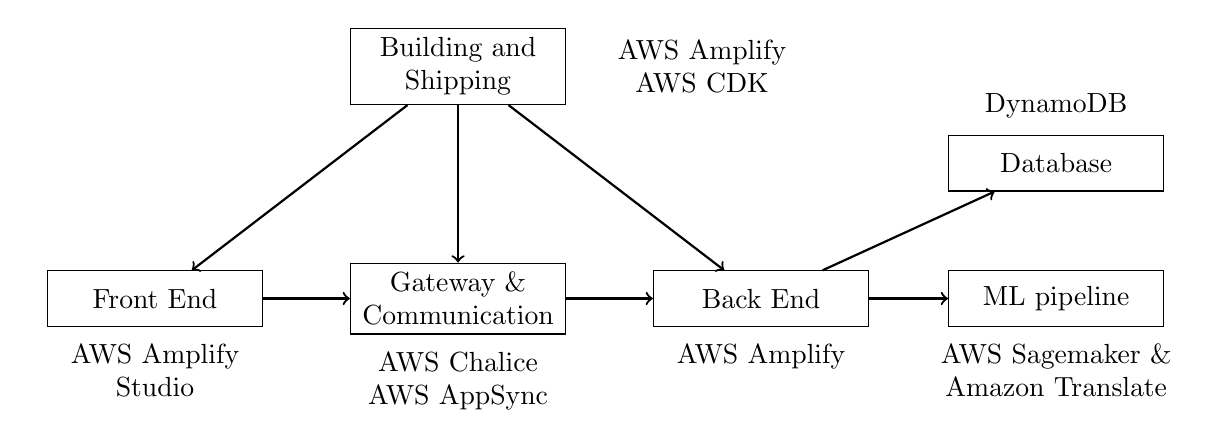
\begin{tikzpicture}[
  block/.style={rectangle, draw, text width=2.5cm, align=center, minimum height=2em},
  arrow/.style={->, thick},
  text_below/.style={align=center, text width=3cm}
]
  \node[block] (building) {Building and Shipping};
  \node[block, below= 2cm of building] (gateway) {Gateway \&\\ Communication};
  \node[block, left = 1.1cm of gateway] (frontend) {Front End};
  \node[block, right = 1.1cm of gateway] (backend) {Back End};
  \node[block, right= 1.1cm and of backend] (ml) {ML pipeline};
  \node[block, above = 1.0 cm of ml] (data) {Database};
  

  \node[text_below, right=0.1cm of building] {AWS Amplify \\ AWS CDK};
  \node[text_below, below=0.1cm of frontend] {AWS Amplify\\Studio};
  \node[text_below, below=0.1cm of gateway] {AWS Chalice \\ AWS AppSync};
  \node[text_below, below=0.1cm of backend] {AWS Amplify};
  \node[text_below, below=0.1cm of ml] {AWS Sagemaker \&\\ Amazon Translate};
  \node[text_below, above=0.1cm of data] {DynamoDB};

  \draw[arrow] (building) -- (frontend);
  \draw[arrow] (building) -- (gateway);
  \draw[arrow] (building) -- (backend);
  \draw[arrow] (backend) -- (ml);
  \draw[arrow] (frontend) -- (gateway);
  \draw[arrow] (gateway) -- (backend);
  \draw[arrow] (backend) -- (data);
  
\end{tikzpicture}
    \caption{Use of AWS services in development}
    \label{fig:Services}
\end{figure}

\subsection{Design Choices}

\indent Figure \ref{fig:rough_sketch} presents the \acrshort{ui} the group has envisioned for the project. We intend for the application to roughly follow this design where we see the original text on the left and translated side on the right. We also intend to give the user the ability to easily translate a different blog post (URL), change the translation language (Language), and the method of translation (Translation). As part of our design, we intend for translations and objects to appear side by side, providing a clear alignment between the original and translated blog.

\indent This initial design is predominantly a product of the client's exact wishes. Claiming that they wanted these exact features visually displayed on the web application. That said, it still follows common design heuristics which are significant to build a bridge between the user and the application to achieve a certain goal \cite{DesignHeuristic}. The design is simplistic, efficient, and the user's has been taken into account, meaning the UI/UX allows for usability of the application on the basis of the user's needs while prioritizing user satisfaction through this feedback cycle \cite{DesignHeuristic}. The accessibility of the application is another important aspect since users with disabilities should be able to use the application as easily as any other user, meaning the final product will follow general \href{https://www.w3.org/TR/WCAG21/}{WCAG2.1} guidelines. 

%%Image of Project Plan
\begin{figure}[ht]
    \centering
    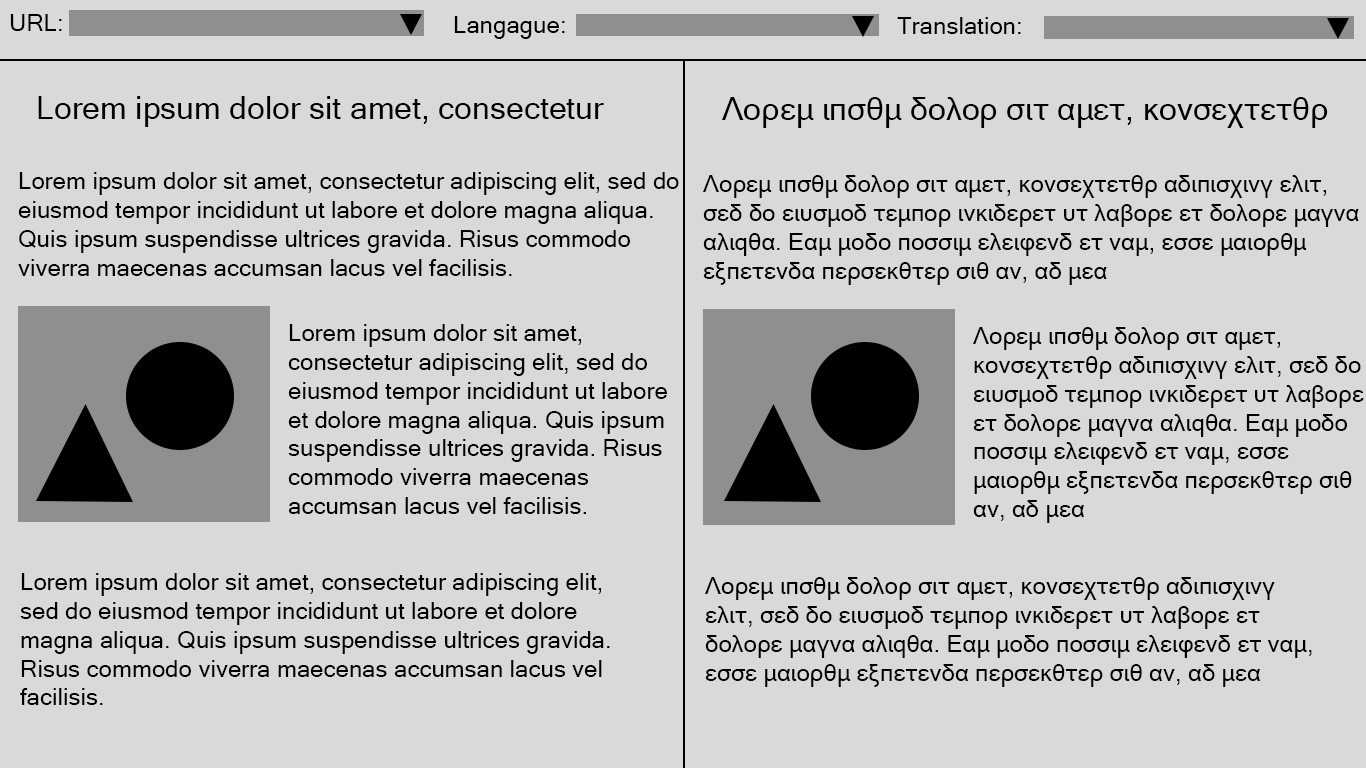
\includegraphics[width=0.8\textwidth]{images/AWS_Blog_translate_rough_sketch.png}
    \caption{Visual Design of Application}
    \label{fig:rough_sketch}
\end{figure}
%%5 Development methodology 
\section{Development Methodology}
\label{sec:developmentmethodology}
%What kind of approach are you using to develop your product (e.g. agile, waterfall)? 
%Section 5.1, 5.2

%What are requirements do you use to accept new functionality? 
%Section 5.1, 5.2

%Do you have a definition of done? 
%Client Notes for external defenition. All Must and should haves and other stuff for internal defenition


%Which tools will you be using for your process?
%AWS tools silly

\subsection{Project Methodology}
\subsubsection{Our Findings}
We have conducted research on four popular development methodologies: Agile, Waterfall, Spiral, and Vee. More of our findings and reasoning behind our choices are in the Appendix, however, for brevity, we have include a bulleted list of the pros and cons of each of these methods.


\begin{itemize}
    \item Agile
    \begin{itemize}
        \item Focus on productivity, flexibility, and practicality \cite{manifest}
        \item Lack of documentation and formal studies
    \end{itemize}
    \item Waterfall
    \begin{itemize}
        \item Document driven, simple, clear-cut milestones \cite{spiralmode;}
        \item Inflexible \cite{spiralmode;}
    \end{itemize}
    \item Spiral
    \begin{itemize}
        \item Iterative planning approach for risk-reduction, with continuously increasing detail \cite{spiralmode;}
        \item Heavy-weight, time-consuming
    \end{itemize}
    \item Vee
    \begin{itemize}
        \item Explicit focus on verification and validation; a lot of testing in mind \cite{geeksforgeeks_2023}
        \item Not very little in the way of implementation, and inflexible \cite{spiralmode;} \cite{geeksforgeeks_2023}
    \end{itemize}
\end{itemize}

\subsubsection{Our Methodology of Choice}

All of the aforementioned models have takeaways that we would like to incorporate in our methodology: iterative refinement of requirements of the Spiral Model, the emphasis on verification and validation from the Vee Model, the explicit documentation and demarcation from the Waterfall method, and the flexibility and iterative implementation approach of Agile. Ideally, we'd like all of these aspects from each of the different frameworks, however, we would not be able to get all of them from simply following any one of them verbatim, so we feel the need to engineer our own hybrid approach, that answers Boehm's questions for process methods: "What shall we do next?" and "How long shall we continue to do it?" \cite[p. 61]{spiralmode;}.

\subsubsection{The Chalice Method}



Trying our best to incorporate all of the aspects from the previous methodologies, and what we discussed with industry experts, we came up with the chalice method, which takes inspiration from all of the aforementioned methods and what AWS practitioners actually use. The area under the blue dashed lines is the \textit{Scrum}; this will occur on a regular basis, very similar to a standard Agile method of implementation. This will keep looping until the team is ready to complete the project. The dotted lines represent back-edges that, ideally, should not be followed, but could be if the project calls for it. Stages outside the \textit{Scrum} subsection are complete when a formal document depicting them is complete, much like the Waterfall method. Stages within the \textit{Scrum} subsection are time-based, with a sprint occurring once a week, much like standard Agile, however, alongside the standard completion criteria that come with Agile, the Chalice method adds a condition, namely, the Software check/ review. For our project, we finish at the Operating and Maintenance stage.


\begin{figure}[h]
    \centering
    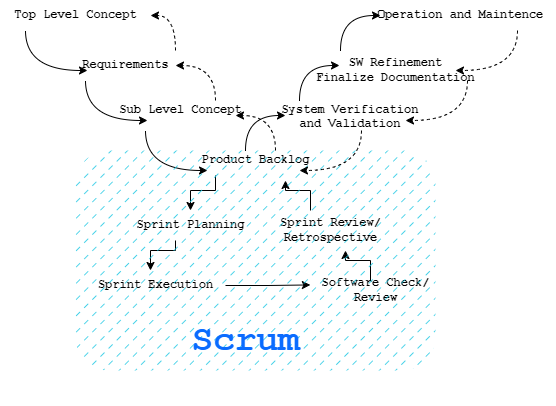
\includegraphics[width=0.7\textwidth]{images/Chalice Method (1).png}
    \caption{The Chalice Method: Alternative to popular methodologies}
    \label{fig:chalice}
\end{figure}

\paragraph*{Top Level Concept (TLC)}
For our project, this part is rather straightforward, it is the grand-scheme concept of what we're building. In this stage, we got introduced to the client, and the project, and selected our low-resource language.

\paragraph*{Requirements}
Similar to the Vee method, this is the stage in which we develop our requirements, and as such, our initial architecture. Based on our highest-level concept, we are able to develop requirements and user stories.

\paragraph*{Sub-Level Concept (SLC)}
Using the requirements, the team is able to come up with a more detailed architecture, which for this project, will give us a solid, detailed foundation and help us select and pinpoint which AWS services we'd really like to use and focus on. Furthermore in this stage, we'd solidify our requirements and technologies, which would lead to a very straightforward implementation approach, since, ideally, all of the architectural kinks should be ironed out during this stage.

\paragraph*{Product Backlog}
This is the first and last stage of the \textit{Scrum} subsection of the model. This replaces the "Implementation" step of the Vee model, giving the team a more rigid framework to actually implement and create the software, based on Agile. Unlike the Vee model, this model is not entirely dependent on previous documentation and different levels of conceptualization to implement the product, instead, this model allows the different concepts to pave the way for the engineers, and create structure, while still allowing them to move freely and make changes within their sprints. This stage has the team examining the product backlog, creating, modifying, and removing user stories and requirements ad-hoc, but at fixed points in the cycle.

\paragraph*{Sprint Planning and Sprint Execution}
These steps are identical to the normal Scrum methodology, wherein our Sprint Plannings are to occur once a week, and our execution is to take place by daily stand-up.

\paragraph*{Software Check/Review}



Based on the conversations we have had with industry experts, we believe, within the Agile-inspired subsection of the Chalice Method, we needed a mechanism specifically designed for receiving feedback and creating documentation, which is where Agile falls short. Our solution to this problem was to modify code reviews frequently found in Agile by also placing emphasis on documentation and code clarity. We perform these modified code reviews at the end of a sprint. Software that meets requirements \textbf{must} pass this step before being complete.


%%

 %In this stage, engineers are put in groups, or partnerships, where they are to briefly examine each others' work, and ensure that other engineers can quickly identify the purpose and the interfaces of their work, and the contributing engineer can quickly justify it with respect to the rest of the system. Ideally, this stage should occur quickly, over the span of about an hour, having everything well documented beforehand, however, if this is not the case, now is the time to fix it. The most significant part of checking the quality of our work is by making sure the translations of the blog posts are accurate. This will be ensured in our weekly meetings with domain experts so that they can assess the quality of the translation and we can improve our service upon this consultation.

%
%
%


\paragraph*{System Verification and Validation}
After a sufficient number of sprints have been completed, the project can move onto the right wall of the chalice, which begins, similar to the Vee method, with the System Verification and Validation stage, where the team ensures that the system as whole works, using various testing methods, and that it meets the requirements.

\paragraph*{SW Refinement and Finalize Documentation}
In this stage, the team ensures that the software is organized and finalizes formal as well as in-line documentation to prepare for the hand-off. If SW refinement occurs, the team may need to take a step back to the previous step.

\paragraph*{Societal Relevance and Ethical Approach}
sIt is not designated in the diagram, however, during the development process of our translation service, we will critically think about the impacts our application could have on society, especially on Native Turkish Speakers. The possible concerns which may arise due to the quality of the application will be kept in mind throughout the development process, and the ethical side of our application will be thought out to make sure we follow the best practices without any negative affect on society. 

\subsection{Communication \& Tools}

As a team, we decided that we will use mainly 3 channels of communication, Discord for online meetings, WhatsApp for general communication, and Mattermost for communication with TAs and the course staff. We use Discord for general meetings related to the project and our daily stand-up sessions where each one of us briefs the entire team on what we, as individuals, have been working on the previous day, what we hope to achieve in the future and ask for clarification or give useful information related to the project and our schedule throughout the meeting. We also have a shared Google Calendar that helps keep us on the same page with regard to the schedule as it is easier than coordinating meetings/deadlines over text communication since it is easy to forget or miss a message. We are also interested in meeting in person, either at AWS’ offices or on campus as we find that we work best as a group when we are all in the same location but we are not sure if working at AWS offices is feasible yet. Furthermore, we use AWS’ internal service, Amazon Chime, to have online meetings with AWS employees. We meet with the technical team at AWS every week on Fridays to discuss our progress and to ask any questions we might have. Furthermore, we will have Gitlab's scrumboard to keep track of our issues as we go .


\section{Design \& Sub Level Concepts}

\indent \indent The application aims to combine eight different AWS services. There include AWS Amplify, AWS AppSync, AWS Lambda, AWS Step Functions, Amazon Translate, AWS SageMaker, Amazon S3, and Amazon DynamoDB. The use of each of these services, and their use in building our application, will be discussed in this section. Overall, in an architecturally complex application with a vast amount of moving parts, the optimal and efficient use of the different AWS service will allow us to have a scalable, accurate and reliable full-stack web application for translating Amazon blog posts.

\subsection{Development and Communication Services}
\textbf{AWS Amplify} is introduced as a development platform for building web applications. AWS Amplify simplifies the development process and facilitates integration with other AWS services, such as Amazon S3 and AWS AppSync. Amplify  allows scalability and security benefits for handling a large number of translation requests and other languages.

\textbf{AWS AppSync}, a fully managed service for developing GraphQL APIs will be used in order to create a GraphQL API that interfaces with translation services. In fact, AWS AppSync can be configured to connect to translation services, such as Amazon Translate, using AWS Lambda for executing the translation logic.

\subsection{Backend Services}
\textbf{AWS Lambda}, a serverless computing service, is the gateway between AWS AppSync and the translation engines. One of Lambda's capabilities is to handle quick computation and incorporate business logic between the gateway and translation engines.

Finally, \textbf{AWS Step Functions}, a serverless workflow service, is as a tool used to orchestrate the translation workflow and managing the flow of data between translation services. Using Step Functions has numerous benefits, including defining dependencies and the ease of managing the application flow using a JSON document.

The architecture of the application starts with \textbf{Amazon DynamoDB}, a serverless and highly scalable NoSQL database, which is chosen as the database for storing the URLs of translated blog posts.

Next, \textbf{Amazon S3} (Simple Storage Service) is introduced as the storage solution for the actual content of translated blog posts. DynamoDB and S3 are integrated to enable efficient storage and retrieval of translated AWS blog posts.

\subsection{Translation and ML Services}
Amazon Translate, a natural language translation service, is discussed as one of the translation modes in the project. The Amazon Translate API is used for translating HTML documents while preserving images and other blog-specific elements. The customization feature of Amazon Translate is also utilised in order to keep technical terms untranslated.

Following is \textbf{Amazon SageMaker}, a platform for machine learning operations, which provides tools for training, testing, deploying, and managing machine learning models. SageMaker is used in data preparation, preprocessing, training, hyperparameter tuning, model evaluation, deployment, inference, monitoring, and iteration processes in order to build a fine-tuned translation model.

\section{Implementation Process}
Process text goes here...
\subsection{Meetings with the Client}
\subsubsection{Requirement elicitation phase}
\subsubsection{Setup phase}
\subsubsection{Implementation phase}
\subsection{Data collection and preprocessing}
\subsection{Integrating Amazon Translate}
\subsection{Building the Machine Learning model}
\section{Development Issues}
\subsection{Version Control}
%Github and Gitlab migration
\subsection{Temporary Account Access}
%AWS account reset -amplify, lambda
\subsection{Access to Blog Post Database}
%Access to data
\section{Testing}
Process text goes here...
\subsection{Testing Frameworks}
\subsection{Manual Testing}
\subsection{Unit Testing}
\subsection{Snapshot Testing}
\subsection{Integration Testing}
\subsection{Acceptance Testing}
\section{Evaluation & Solution}
\subsection{Translation Quality}
\subsection{Comparison of the two approaches}
\section{Ethics and Values}

\subsection{Ethical Approach}
\subsection{Societal impact of our application}
\subsection{Possible outcomes resulting from our application}

\indent \indent Our full-stack web application uses two different types of translation services: Amazon Translate and our own transformer-based translation model trained on a data set consisting of manually translated Amazon Web Service blog posts. Due to our application relying heavily on machine learning models in order to translate blog posts from English to Turkish, there is room for ethical concern when working with these models. 

\indent The translations completed by our model are important to increase the accessibility of information to native Turkish speakers. Through the use of this service, these users should be able to access the same information as any other user that is proficient in a high-resource language. The quality of the translation that our model outputs has a high impact on the user's ability to understand the blogposts; a high-quality translation service will increase user satisfaction and experience by allowing more users access to significant technical information residing in the blog posts. In the case that we achieve a good translation model, more users will be reached through AWS markets which will have a mutually beneficial outcome for our client as well as AWS customers/users. However, in the case that we achieve a low-quality translation, these users will not be given access to important information that they should have. 

\indent Although we will be training our model on a manually translated data set, it is significant to consider the difficulties regarding translating English to Turkish since we may not be able to catch the accurate meaning of the sentences with the limited data set we have. Inaccurate translations have the potential to be harmful to users who wish to acquaint themselves with information regarding AWS in terms of time and cost (for example, our model could inaccurately translate the way an AWS service works, leading to time and possible money lost as the user who is reading the blog could carry this mistake over into their work). 

In general, we have found that our translation model does not pose much of a concern regarding human rights and values as our model is intended to only work with AWS blog posts that mostly remain technical and related to AWS Services, so there is little room for dangerous translations. Furthermore, since our application is very connected to user experience, before our finished product, we will do acceptance testing to ensure the quality of our translation as well as a good user experience. We will try to improve our translation by gathering more training data from other resources to strive for a high-quality translation service.  

\section{Conclusion}

\newpage
\clearpage

\bibliography{ref}

\newpage
\clearpage
\pagenumbering{alph}

\begin{appendices}
    \section{Research on Methodologies}
\subsection{Agile}
As software engineers from TU Delft, we've been taught to use Agile methods, specifically, the Scrum method, wherein engineers create a feedback loop based on what has been done, and what needs to be done, having regular meetings where progress is reviewed, and brief planning is done for the near future. In most Agile methods, immediate productivity and risk reduction are put to the forefront, which, specifically in the Scrum method takes, place through constant meetings with the client and with the teams, to assess difficulties, changes in requirements, and specifications, all in the name of reducing risks with regards to the final product \cite{agilesource}. Following the release of the \href{https://agilemanifesto.org/}{Manifesto for Agile Software Development}, these methods have become highly popular, as they stray away from the previously bloated, long-winded development models, such as the Waterfall \cite{manifest}. Agile methods are practical, as they focus on simplicity, constantly working software, and welcome changes in the specifications or requirements \cite{beck2001agile}. This is where Agile methods strive: simply producing results in environments where the engineers just have to make a working system, however, we find that there are some limitations to Agile and its simple, incremental style. The lightweight framework, although very efficient for simply writing code, has little in the way of documentation, prototyping, and formal studies, making the steps following production (operating, maintenance, and deployment) potentially more difficult than they have to be. As our client is an extremely large company, and they've explicitly mentioned that they hope to continue maintaining, modifying, and deploying our system after we have finished, we find the steps after \textbf{our} production life-cycle to be extremely important. For this reason, among others, we explored alternatives to Agile \cite{relation}.

\subsection{Waterfall}
The Waterfall model is a process method that, recently, has been less popular due to the rise of practicality-focused Agile methods, however, its apparent decline in popularity does not mean it is necessarily inferior. The Waterfall model belongs to a class of process models called Document-driven models, which, contrary to Agile models, have clearly defined stages, which are demarcated by detailed documents \cite{spiralmode;}. Although some may not see the value in spending time creating documents for each stage, having documentation to reference later on, whether it be for the same team, new members, or different team picking up where another left off, documentation, especially depicting choices in design are an invaluable resource, which is often not given explicit time in Agile methods. Furthermore, the Waterfall method is linear, assuming that each steps occur one after the other and that teams often shouldn't have to go back, unless something goes wrong. Given that we intend to make a robust system to hand off to AWS after the completion of this project, detailed documents after each are extremely useful. This methodology also has extremely clear milestones, which, although there will not be a working system at each step, the client will have some sort of idea of how the project is going with the documents. Despite this, the Waterfall model certainly isn't perfect. Given the robust and sequential nature of the model, it is rather inflexible, as changes to the requirements, according to the model, are not able to be accounted for without going back and editing every after the first one that was changed. Furthermore, since prototyping and experimentation don't occur until later, errors may be detected rather late, which, given the short-lived nature of this project, we certainly cannot afford \cite{comparitvestudy}.

\begin{figure}[H]
\centering
\begin{subfigure}{0.5\textwidth}
  \centering
  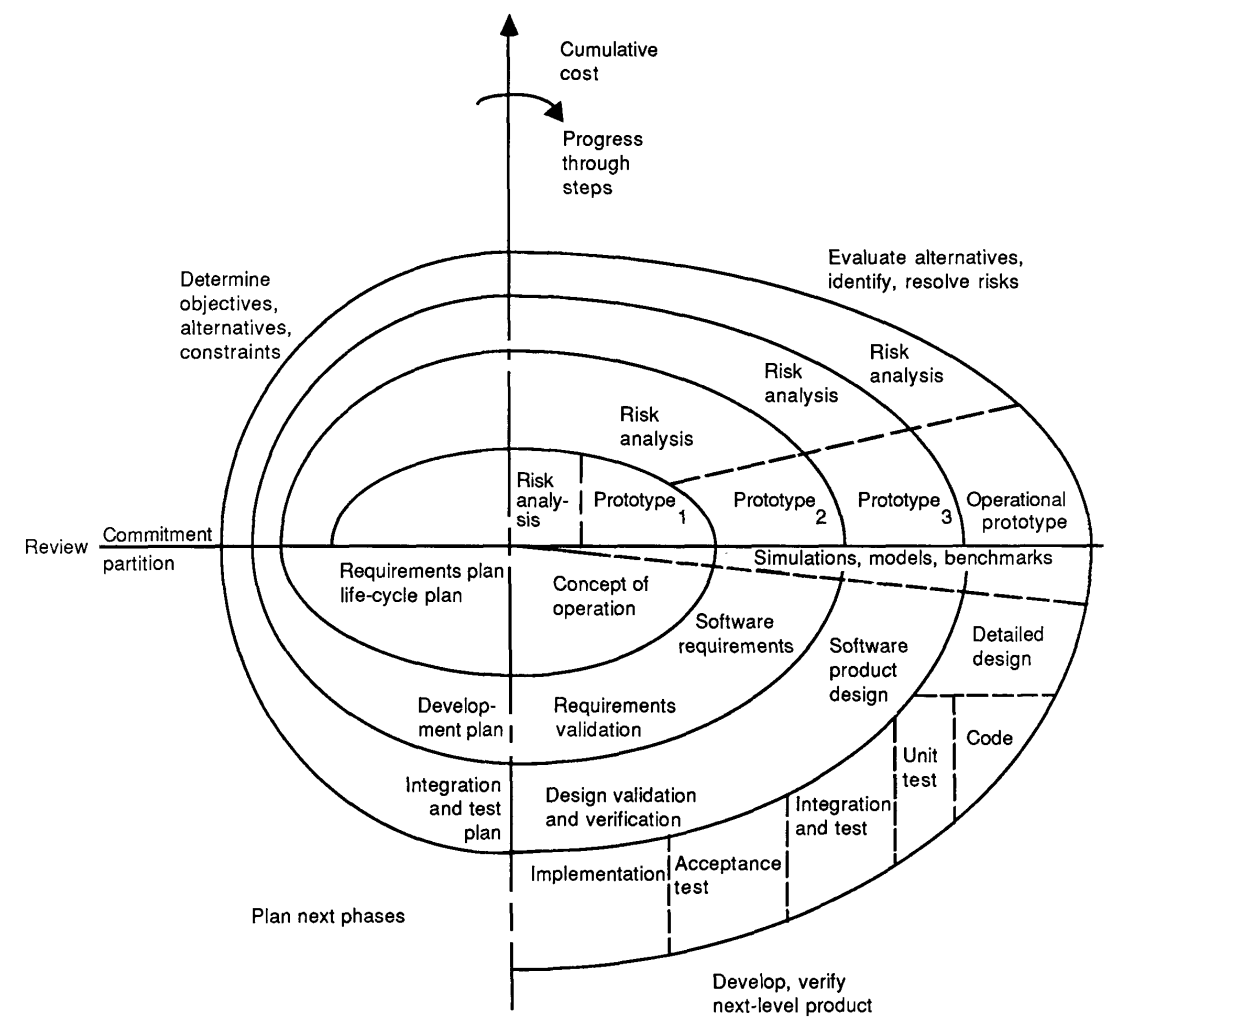
\includegraphics[width=.4\linewidth]{images/Spiral Model.png}
  \caption{Spiral model \cite{spiralmode;}}
  \label{fig:sub1}
\end{subfigure}%
\begin{subfigure}{0.5\textwidth}
  \centering
  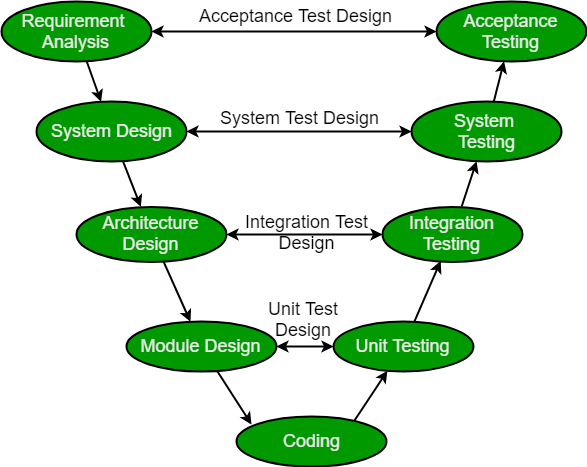
\includegraphics[width=.4\linewidth]{images/vee.png}
  \caption{Vee model \cite{geeksforgeeks_2023}}
  \label{fig:sub2}
\end{subfigure}
\caption{The Spiral and Vee models side by side}
\label{fig:test}
\end{figure}

\subsection{Waterfall Derivatives: Spiral and Vee}
From the Waterfall model, came many improvements, the two most notable that we have considered are the Vee model and the Spiral model \cite{spiralmode;} \cite{geeksforgeeks_2023}. The spiral model builds on top of the Waterfall by creating an iterative approach in the planning phase, wherein each phase risks are assessed and analyzed, a prototype is created, and more information is contextualized for the next phase, making the successive iterations more detailed, yet time-consuming. This model does not appear to have much in the way of dictating how the implementation steps are to be carried out, as by the time actual implementation is to occur, the documents depicting the software should have been already written, with only the fine-grained details being necessary for the final spiral. Alternatively, for our purpose, the prototypes could be adapted for high-level iterations toward the final working product. The Vee Model builds on top of the Waterfall model by being linear, however, adds explicit many explicit verification and validation steps. The model suggests that software engineering is at the highest level, verifying the requirements at each step, and then after code completion, through testing, work its way back up, going through steps of unit testing, integration testing, etc. \cite{geeksforgeeks_2023}. These validation steps work in tandem with the verification steps in terms of abstraction, ensuring that they meet and align with each other, oftentimes being done in parallel. With all this information in mind, it is important to remember the purpose of a process model: "Thus, a process model addresses the following software project questions: (1) What shall we do next? (2) How long shall we continue to do it. \cite{spiralmode;}"

\end{appendices}


\end{document}